% Chapter Template

\chapter{Ensayos y resultados} % Main chapter title

\label{Chapter4} % Change X to a consecutive number; for referencing this chapter elsewhere, use \ref{ChapterX}
En este capítulo se presentan los resultados obtenidos de los ensayos realizados, que incluyen, pero no se limitan a: resultado de la segmentación CNN U-Net para la obtención de la serie temporal de superficie de agua de la laguna, resultados de modelado SARIMA para todas las series temporales estudiadas, resultado del modelado VAR y, por último, los resultados de la aplicación de rolling forecasting a las variables área. 

%----------------------------------------------------------------------------------------
%	SECTION 1
%----------------------------------------------------------------------------------------

\section{Segmentación mensual con U-Net: resultados operativos}

La segmentación automática de cuerpos de agua se implementó con una arquitectura U-Net entrenada bajo el esquema \textit{student–teacher}. El objetivo fue obtener una serie mensual continua de cobertura de agua superficial, evitando la necesidad de etiquetado manual masivo. Para ello, se empleó un 5\% de las imágenes del cubo temporal mensual, generando las etiquetas a partir del NDWI umbralizado (>0,15). El modelo resultante se aplicó a la totalidad de imágenes del período 1984–2022.

\subsection{Curvas de entrenamiento y validación}
En la figura~\ref{fig:unet_training} se muestran las curvas de entrenamiento y validación de la red U-Net, utilizando \textit{Binary Cross Entropy} (BCE) como función de pérdida. Se observa una disminución rápida de dicha pérdida durante las primeras 15 épocas, seguida de una convergencia estable hacia valores próximos a cero. La similitud entre las curvas de entrenamiento y validación indica un buen equilibrio entre ajuste y generalización. El mejor desempeño en validación se alcanzó en la época 78, lo que confirma la capacidad del modelo para segmentar de manera consistente las áreas de agua a partir de las imágenes Landsat.

\begin{figure}[H]
    \centering
    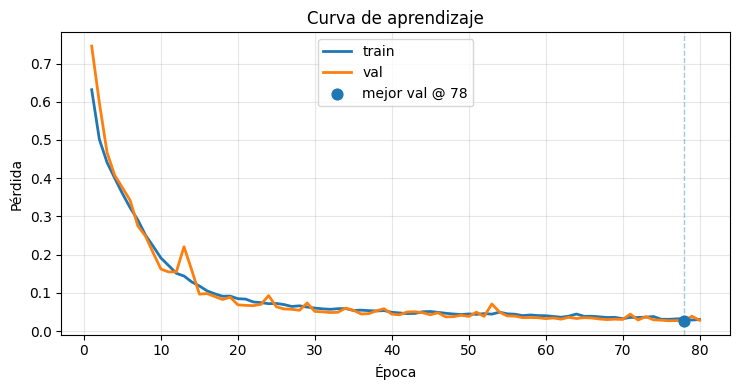
\includegraphics[scale=0.55]{Figures/curva_entrenamiento.png}
    \caption{Curvas de entrenamiento y validación de la U-Net.}
    \label{fig:unet_training}
\end{figure}

\subsection{Ejemplos de segmentación}
La figura~\ref{fig:unet_examples} muestra ejemplos representativos de la segmentación mensual: a la izquierda las imágenes Landsat en composición RGB de falso color, y a la derecha las máscaras binarias generadas por la U-Net. Se aprecia coherencia espacial en la identificación de cuerpos de agua, con detección consistente de la laguna central y reducción de falsos positivos respecto de umbrales simples de NDWI.

\begin{figure}[H]
    \centering
    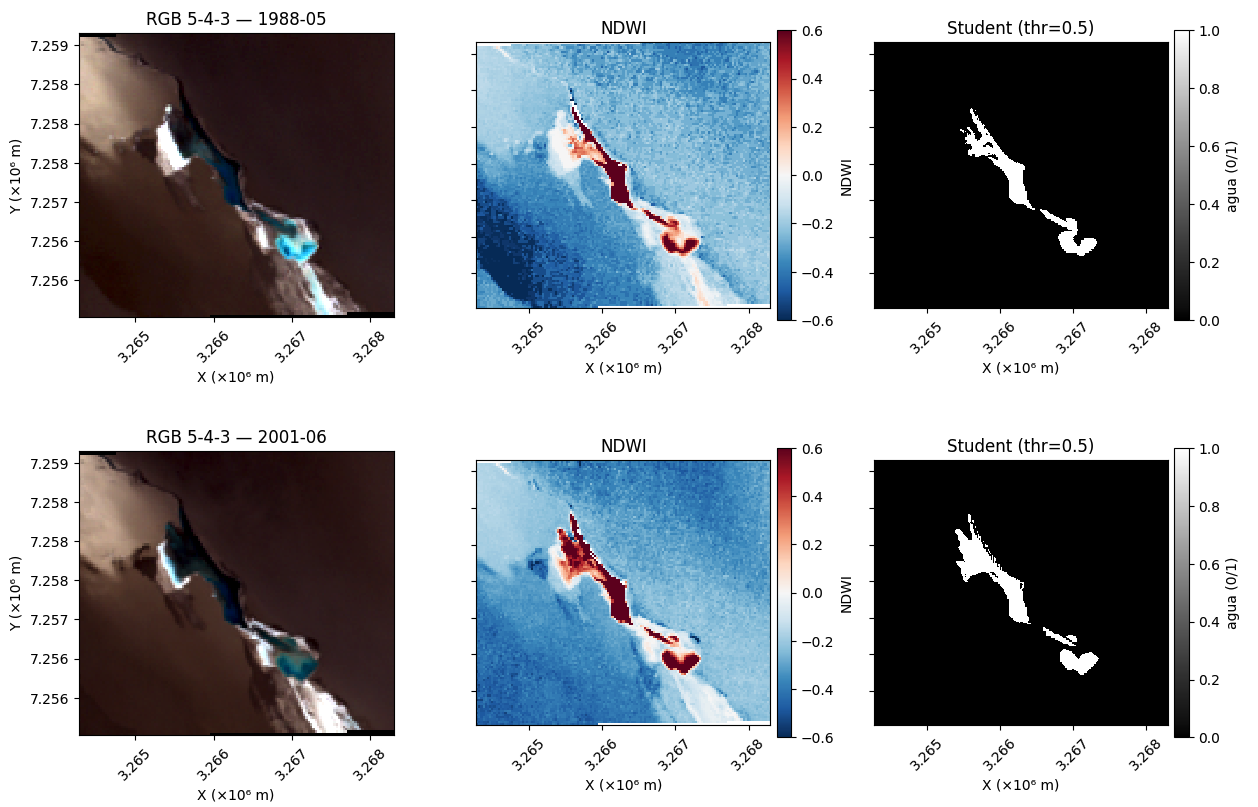
\includegraphics[scale=0.31]{Figures/unet_examples.png}
    \caption{Ejemplos de segmentación mensual: comparación entre imágenes Landsat (falso color) y máscaras U-Net.}
    \label{fig:unet_examples}
\end{figure}

\subsection{Probabilidad mensual de agua}

A partir del cubo temporal clasificado con la U-Net se calculó, para cada mes del período de análisis, la probabilidad de ocurrencia de agua. Este cálculo se realizó como la proporción de píxeles clasificados como agua sobre el total de píxeles de la laguna en el mes correspondiente. De esta manera, se obtuvo una serie temporal mensual de probabilidades que permite evaluar la consistencia del modelo y la dinámica hidrológica en escalas estacionales e interanuales.

En la figuras~\ref{fig:prob_agua_mensual} y figura~\ref{fig:prob_agua_mensual2} se presentan ejemplos gráficos de estos resultados. Se observa la variabilidad temporal de la probabilidad de agua, con máximos que coinciden con períodos de mayor extensión superficial y mínimos en fases de retracción. Este producto constituye un insumo clave para la modelización temporal desarrollada en los capítulos siguientes, pues resume la dinámica de la laguna en una métrica probabilística derivada de la clasificación automática.

\begin{figure}[H]
    \centering
    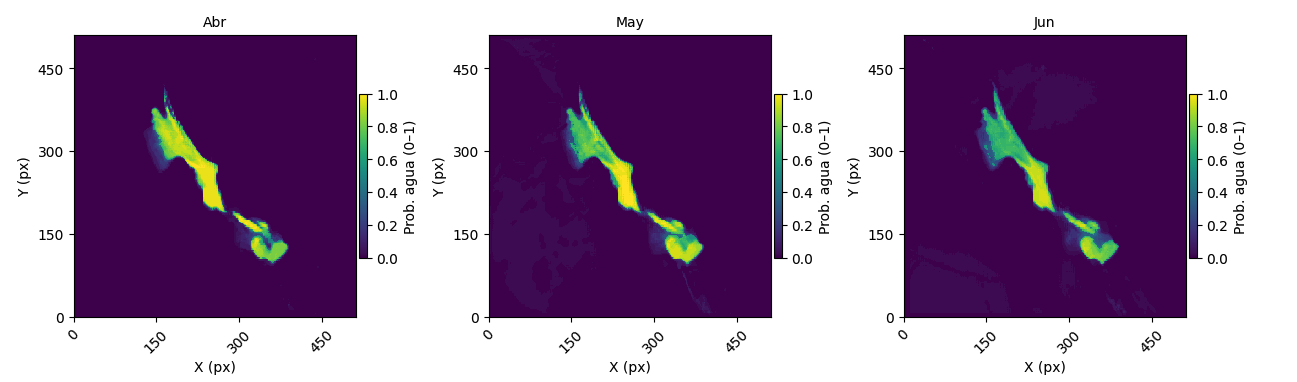
\includegraphics[scale=0.31]{Figures/prob_agua1.png}
    \caption{Probabilidad mensual de ocurrencia de agua en la laguna Llullaillaco, derivada de la segmentación U-Net.}
    \label{fig:prob_agua_mensual}
\end{figure}

\begin{figure}[H]
    \centering
    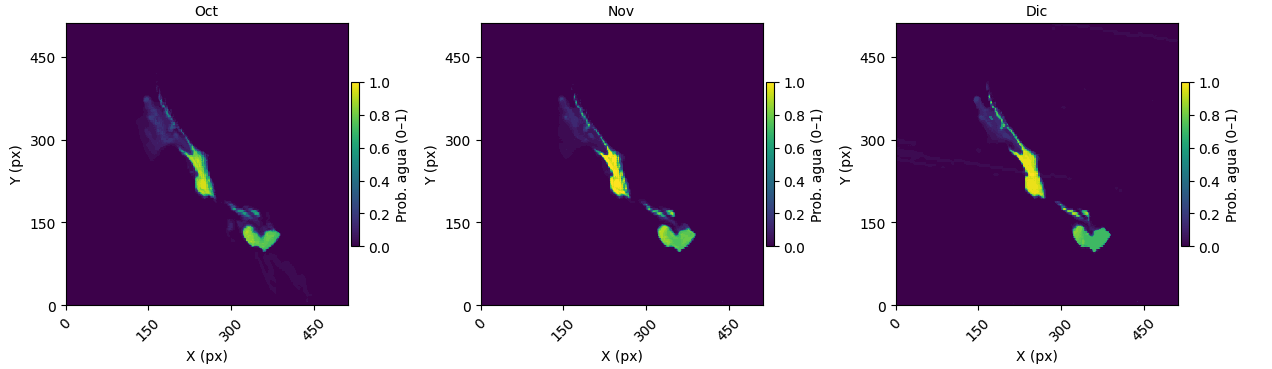
\includegraphics[scale=0.31]{Figures/prob_agua2.png}
    \caption{Probabilidad mensual de ocurrencia de agua en la laguna Llullaillaco, derivada de la segmentación U-Net.}
    \label{fig:prob_agua_mensual2}
\end{figure}

\section{Modelado con SARIMA}

El modelo SARIMA (\textit{Seasonal ARIMA}) fue optimizado para cada una de las series de interés (ONI, SOI, MEI y \texttt{Área}), evaluando diferentes combinaciones de parámetros $(p,d,q)\times(P,D,Q,s)$ y seleccionando los mejores ajustes según el criterio de información de Akaike (AIC). 

\subsection{Variable ONI}
El mejor modelo seleccionado para ONI fue SARIMA$(2,0,1)\times(1,1,2)_{12}$, con un AIC de $-410.64$. Este modelo supera en desempeño a alternativas cercanas como SARIMA$(2,0,2)\times(1,1,2)_{12}$ y SARIMA$(2,0,0)\times(1,1,2)_{12}$ y confirma que la estructura óptima incluye un componente autorregresivo de orden 2 y un componente de media móvil de orden 1.

\subsection{Variable SOI}
En el caso de SOI, el mejor modelo corresponde a SARIMA$(1,0,2)\times(2,1,2)_{12}$, con un AIC de $2842.34$. Aunque este valor absoluto es elevado (debido a la alta varianza intrínseca de la serie), la comparación relativa muestra que es la configuración más adecuada frente a otras alternativas con órdenes similares.

\subsection{Variable MEI}
La serie MEI fue mejor explicada por SARIMA$(2,0,2)\times(1,1,2)_{12}$, y alcanzó un AIC de $126.37$. Este modelo captura tanto la persistencia como los patrones estacionales de la serie, y presenta una ventaja clara frente a otros candidatos como SARIMA$(1,0,1)\times(1,1,2)_{12}$ y SARIMA$(2,0,1)\times(1,1,2)_{12}$.

\subsection{Variables Área y Área\_diff}
Para la serie \texttt{Área} sin diferenciar, el mejor modelo fue SARIMA$(1,0,0)\times(1,0,1)_{12}$ con un AIC de $-902.08$. Sin embargo, al diferenciar la serie (\texttt{Área\_diff}), se obtuvo como mejor ajuste el modelo SARIMA$(2,0,1)\times(1,0,1)_{12}$ con un AIC de $-888.19$. Aunque el AIC es ligeramente menos favorable tras la diferenciación, los análisis de raíces unitarias y métricas de predicción (ver subsección anterior) mostraron que el modelo diferenciado ofrece mayor robustez y estacionariedad.

\begin{table}[H]
    \centering
    \caption{Resumen de los mejores modelos SARIMA seleccionados por serie.}
    \begin{tabular}{lccc}
        \toprule
        \textbf{Serie} & \textbf{Mejor modelo SARIMA} & \textbf{AIC} & \textbf{Notas} \\
        \midrule
        ONI   & $(2,0,1)\times(1,1,2)_{12}$ & $-410.64$ & Estacionalidad marcada \\
        SOI   & $(1,0,2)\times(2,1,2)_{12}$ & $2842.34$ & Alta varianza residual \\
        MEI   & $(2,0,2)\times(1,1,2)_{12}$ & $126.37$  & Buen equilibrio AR y MA \\
        Área  & $(1,0,0)\times(1,0,1)_{12}$ & $-902.08$ & No diferenciada \\
        Área\_diff & $(2,0,1)\times(1,0,1)_{12}$ & $-888.19$ & Estacionaria, mayor robustez \\
        \bottomrule
    \end{tabular}
    \label{tab:sarima_modelos}
\end{table}

En síntesis, el procedimiento de optimización permitió identificar configuraciones distintas para cada serie, adaptadas a sus características temporales, ver tabla \ref{tab:sarima_modelos}. En los siguientes apartados se evaluará la performance predictiva de estos modelos sobre los conjuntos de test.

\section{Evaluación de los modelos SARIMA}

Se evaluó el desempeño predictivo de los modelos SARIMA seleccionados para las series
ONI, SOI, MEI, \texttt{Área} y \texttt{Área\_diff}, considerando: métricas de error en el
conjunto de test (MSE, MAE, RMSE y MAPE cuando aplica), diagnóstico de residuos
(residuos en el tiempo, ACF/PACF de residuos, normalidad aproximada y test de Ljung--Box),
y parsimonia y significancia de coeficientes (AIC/BIC, $p$--valores).

\subsection{Criterios de diagnóstico}
Se consideró que un modelo es adecuado cuando:
\begin{itemize}
    \item los residuos no presentan autocorrelación remanente (ACF/PACF dentro de bandas y Ljung--Box con $p>0.05$),
    \item no hay patrones sistemáticos en los residuos,
    \item las métricas de error son coherentes con la escala de la serie,
    \item la parametrización es parsimoniosa (sin términos innecesarios o no significativos).
\end{itemize}

\subsection{Resultados por serie y diagnóstico}
En el apéndice de figuras \ref{AppendixA} se incluyen los siguientes gráficos y resultados:

\begin{itemize}
    \item Residuos en el tiempo.  
    \item Funciones de autocorrelación (ACF) y autocorrelación parcial (PACF) de los residuos.  
    \item Histograma, densidad y gráfico Q--Q.  
    \item Gráfico de p--valores de la prueba de Ljung--Box por rezago.  
    \item Serie observada (train+test) versus predicciones con intervalo de confianza al 95\%.  
\end{itemize}

\subsubsection{Evaluación de la serie ONI} 
El análisis se llevó a cabo con el modelo SARIMA$(2,0,1)\times(1,1,2)_{12}$ (AIC $\approx -410.6$). 
Los coeficientes no estacionales AR(2) y MA(1) resultaron altamente significativos, lo que permitió capturar de manera adecuada la dinámica de corto plazo. En contraste, los términos estacionales no alcanzaron significancia estadística. El test de Jarque--Bera rechazó la hipótesis de normalidad y se detectó heterocedasticidad; sin embargo, los residuos no mostraron autocorrelaciones relevantes.  
En el conjunto de datos de prueba, las métricas de desempeño fueron MSE $=0.683$, MAE $=0.631$ y RMSE $=0.826$. En las figuras~\ref{fig:res_oni} y~\ref{fig:pred_oni} se ilustran los residuos del modelo y las predicciones sobre el set de test.  

Observación: el modelo logra un buen ajuste de la dinámica no estacional; se recomienda simplificar la parte estacional (evaluar un ARIMA$(2,0,1)$ sin componente estacional) y volver a examinar los residuos.  
\vspace{0.3em}


\subsubsection{Evaluación de la serie SOI}
El análisis de la serie SOI se realizó mediante el modelo SARIMA$(1,0,2)\times(2,1,2)_{12}$ (AIC $\approx 2116$). 
Los parámetros AR(1), MA(1) y varios términos estacionales resultaron significativos, mientras que el MA(2) y el AR estacional a 24 meses no lo fueron. Los residuos no evidenciaron autocorrelación (test Ljung--Box con $p>0.05$), aunque presentaron una ligera desviación respecto de la normalidad.  
En el conjunto de prueba, las métricas obtenidas fueron MSE $=88.00$, MAE $=7.64$ y RMSE $=9.38$. Las figuras~\ref{fig:res_soi} y~\ref{fig:pred_soi} muestran tanto los residuos como las predicciones en el set de validación.  

Observación: el modelo presenta un desempeño predictivo limitado en relación con la escala del SOI. Resulta conveniente simplificar la estructura, eliminando términos no significativos y explorando transformaciones más robustas.  
\vspace{0.3em}


\subsubsection{Evaluación de la serie MEI}
La serie MEI fue modelada mediante un SARIMA$(2,0,2)\times(1,1,2)_{12}$ (AIC $\approx 126.4$). 
Los coeficientes no estacionales AR(1), AR(2) y MA(1) mostraron gran significancia, mientras que MA(2) se comportó de manera marginal. En la componente estacional, únicamente el término AR a 12 meses resultó relevante, mientras que los términos MA estacionales no aportaron significativamente. Los residuos no evidenciaron autocorrelación (Ljung--Box con $p\approx 0,84$), aunque presentaron colas algo pesadas.  
En el conjunto de prueba se obtuvieron las métricas: MSE $=0.821$, MAE $=0.725$ y RMSE $=0.906$. Las figuras~\ref{fig:res_mei} y~\ref{fig:pred_mei} presentan los residuos y las predicciones sobre el set de test.  

Observación: el modelo ofrece un desempeño predictivo sólido. En futuros trabajos sería apropiado simplificar la parte estacional (p.\,ej., SARIMA$(2,0,1)\times(1,1,0)_{12}$) y revisar nuevamente el comportamiento de los residuos.  
\vspace{0.3em}


\subsubsection{Evaluación de la serie Área (sin diferenciar)}
La serie \texttt{Área}, sin diferenciación, se ajustó con un modelo SARIMA$(1,0,0)\times(1,0,1)_{12}$ (AIC $\approx -902.1$). 
Todos los coeficientes estimados resultaron significativos, destacándose un coeficiente AR estacional elevado ($\approx 0.996$), lo que sugiere la conveniencia de considerar diferenciación estacional. Los residuos no mostraron autocorrelaciones relevantes, aunque presentaron cierta desviación respecto de la normalidad.  
En el conjunto de datos de prueba, los resultados fueron MSE $=0.02499$, MAE $=0.119$ y RMSE $=0.158$. Las figuras~\ref{fig:res_area} y~\ref{fig:pred_area} ilustran tanto los residuos como las predicciones generadas por el modelo.  

Observación: el ajuste es adecuado en la escala de la serie; no obstante, la elevada magnitud del AR estacional sugiere evaluar un $D=1$ para garantizar mayor estabilidad.  
\vspace{0.3em}


\subsubsection{Evaluación de la serie Área\_diff (diferenciada)}
Finalmente, para la serie diferenciada \texttt{Área\_diff}, se aplicó un modelo SARIMA\\$(2,0,1)\times(1,0,1)_{12}$ (AIC $\approx -888.2$). 
Los residuos se comportaron como ruido blanco (ACF/PACF dentro de las bandas de confianza, Ljung--Box con $p>0,05$), presentando además una distribución cercana a la normalidad.  
En el conjunto de prueba, el desempeño fue particularmente destacable: MSE $=0.01782$, MAE $=0.0910$, RMSE $=0.1335$ y MAPE $=1.70\%$. En las figuras~\ref{fig:res_area_d} y~\ref{fig:pred_area_d} se visualizan los residuos y las predicciones en el set de test.


Observación: el modelo muestra un comportamiento predictivo muy satisfactorio. A futuro, podría considerarse una estructura aún más parsimoniosa y realizar verificaciones adicionales de los residuos.  
\vspace{0.3em}



En la tabla~\ref{tab:metricas_sarima} se pueden observar las métricas para los modelos SARIMA para variables analizadas. 

\begin{table}[H]
\centering
\caption{Resumen de métricas de desempeño en test para modelos SARIMA.}
\label{tab:metricas_sarima}
\begin{tabular}{lcccc}
\toprule
\textbf{Serie} & \textbf{MSE} & \textbf{MAE} & \textbf{RMSE} & \textbf{MAPE} \\
\midrule
ONI  & 0,683  & 0,631  & 0,826  & n/a \\
SOI  & 88,003 & 7,639  & 9,381  & n/a \\
MEI  & 0,821  & 0,725  & 0.906  & n/a \\
Área (sin diff) & 0,02499 & 0,1190 & 0,1581 & n/a \\
Área\_diff      & 0,01782 & 0,0910 & 0,1335 & 1,70\% \\
\bottomrule
\end{tabular}
\end{table}

A continuación se sintetizan los principales hallazgos asociados a la aplicación del modelo SARIMA en las series temporales:

\begin{itemize}
    \item Series ENSO (ONI, MEI): los componentes AR(2) y MA(1) no estacionales
    capturan bien la memoria de corto plazo; varios términos MA estacionales no son
    significativos.
    \item Serie SOI: los residuos no muestran autocorrelación, las métricas de la precisión predictiva son altas.
    \item Series \texttt{Área} vs. \texttt{Área\_diff}: ambos modelos presentan muy buen desempeño en test,
    destacándose \texttt{Área\_diff} con los errores más bajos y residuos más
    estables.
\end{itemize}

En conjunto, la evidencia empírica muestra que la diferenciación de la serie \texttt{Área}
mejora la robustez y precisión del modelo, mientras que en las series ENSO una
parametrización más parsimoniosa tiende a ser suficiente. El caso SOI requiere trabajo
adicional para alcanzar niveles de error aceptables.

\section{Modelado VAR (vectores autorregresivos)}

El modelo VAR (\textit{Vector AutoRegressive}) es una técnica de series temporales multivariadas que permite capturar las interdependencias entre varias variables a lo largo del tiempo. A diferencia de los modelos univariados como ARIMA o SARIMA, el VAR considera que cada variable del sistema depende no solo de sus propios valores pasados, sino también de los valores pasados de las demás variables incluidas en el modelo \parencite{lutkepohl2005new}.

El análisis VAR constituye la base para explorar relaciones causales entre las variables y evaluar la capacidad predictiva conjunta del sistema.

\subsection{Prueba de causalidad de Granger}

La prueba de causalidad de Granger evalúa si los valores pasados de una serie temporal contienen información útil para predecir otra serie, bajo el supuesto de relaciones lineales dentro de un modelo VAR \parencite{granger1969investigating}.
La hipótesis nula (\(H_0\)) establece que “la serie X no causa Granger a la serie Y”. Un p-valor inferior a 0,05 permite rechazar la hipótesis nula, concluyendo que existe causalidad grangeriana.

En este estudio, se aplicó la prueba con un máximo de 24 rezagos mensuales, y se obtuvo la matriz de resultados presentada en la tabla~\ref{tab:granger_matrix}.

\begin{table}[H]
    \centering
    \caption{Matriz de p-valores de la prueba de causalidad de Granger (máx. 24 rezagos).}
    \label{tab:granger_matrix}
    \begin{tabular}{lcccc}
        \toprule
        & ONI\_x & SOI\_x & MEI\_x & Área\_x \\
        \midrule
        ONI\_y  & 0,9999   & 0,1189   & 0,0142$^{*}$ & 0,1057   \\
        SOI\_y  & 0,0000$^{*}$ & 1,0000   & 0,0000$^{*}$ & 0,0410$^{*}$ \\
        MEI\_y  & 0,0000$^{*}$ & 0,0000$^{*}$ & 1,0000   & 0,3261   \\
        Área\_y & 0,5889   & 0,0456$^{*}$ & 0,4557   & 1,0000   \\
        \bottomrule
    \end{tabular}
    \vspace{0.2cm}
    
    \raggedright \footnotesize{$^{*}$ Significativo al nivel del 5\% (p $<$ 0,05).}
\end{table}

A continuación se presenta una síntesis de los principales hallazgos obtenidos por la prueba de causalidad de Granger:
\begin{itemize}
    \item ONI\_y: solo es causado por el MEI (p=0,014), lo que indica que la información del índice multivariado MEI contribuye a predecir al ONI.
    \item SOI\_y: recibe causalidad de ONI, MEI y el \texttt{Área}y refleja su carácter central como índice atmosférico.
    \item MEI\_y: es causado por ONI y SOI, lo que confirma la fuerte interdependencia entre los índices climáticos de ENSO.
    \item Área\_y: solo es causada por el SOI (p=0,046), lo que evidencia que la variabilidad atmosférica influye directamente en la superficie de agua del salar.
\end{itemize}


El análisis de causalidad de Granger confirma la interdependencia entre los tres índices climáticos (ONI, SOI, MEI), coherente con la naturaleza multivariada del ENSO. Entre ellos, el SOI emerge como el índice más influyente, pues no solo se ve afectado por ONI y MEI, sino que además es el único que causa variaciones significativas en el área de agua superficial. Este hallazgo refuerza la hipótesis de que la dinámica atmosférica vinculada al SOI constituye un modulador clave de la hidrología altoandina.

\subsection{Modelo VAR: selección del orden y resultados}

Para modelar la dinámica conjunta entre los índices ENSO (ONI, SOI, MEI) y la superficie de agua (\texttt{Área}), se ajustó un modelo VAR. A diferencia de los modelos univariados como ARIMA o SARIMA, el VAR permite capturar relaciones dinámicas multivariadas, considerando que cada variable depende tanto de sus propios rezagos como de los rezagos de las demás variables del sistema \cite{lutkepohl2005new}.

\subsubsection{Selección del orden de rezagos}
Se evaluaron los criterios de información AIC, BIC, HQIC y FPE para determinar el número óptimo de rezagos (tabla~\ref{tab:var_lags}). Los resultados muestran que el rezago $p=3$ minimiza la mayoría de los criterios (AIC, HQIC y FPE), por lo que se seleccionó un modelo VAR(3).

\begin{table}[H]
    \centering
    \begin{threeparttable}
    \caption{Selección del orden de rezagos para el modelo VAR.}
    \label{tab:var_lags}
    \begin{tabular}{lcccc}
        \toprule
        \textbf{Rezago} & \textbf{AIC} & \textbf{BIC} & \textbf{HQIC} & \textbf{FPE} \\
        \midrule
        2 & -7,485 & -7,130\tnote{*} & -7,345 & 0,0005612 \\
        3 & -7,617\tnote{*} & -7,104 & -7,414\tnote{*} & 0,0004921\tnote{*} \\
        \bottomrule
    \end{tabular}
    \begin{tablenotes}
      \footnotesize
      \item [*] * Significativo al nivel del 5\% (p $<$ 0,05).
    \end{tablenotes}
    \end{threeparttable}
\end{table}


El ajuste del modelo mostró que:

\begin{itemize}
    \item ONI presenta un fuerte componente autoregresivo, con significancia en los rezagos 1 y 3, lo que confirma su persistencia temporal.
    \item SOI depende de sus propios rezagos, pero también recibe influencia significativa del ONI, reforzando los vínculos entre estos índices ENSO.
    \item MEI es explicado principalmente por sus propios rezagos, aunque también recibe influencia de ONI y SOI.
    \item El \texttt{Área} muestra alta dependencia de su propio rezago inmediato (L1.Area $\approx 0,67$), lo que indica fuerte persistencia temporal. Además, se observa una influencia marginal de SOI (p$\approx 0,05$), consistente con la prueba de causalidad de Granger.
\end{itemize}

Por otra parte, la matriz de correlación entre los residuos (tabla~\ref{tab:var_corr_resid}) muestra que:

\begin{itemize}
    \item ONI y MEI presentan una correlación positiva alta (0,59), consistente con la interdependencia observada en los coeficientes.
    \item SOI mantiene correlaciones negativas con ONI (-0,23) y MEI (-0,45), reforzando su rol como índice atmosférico diferenciado.
    \item El \texttt{Área} muestra correlaciones débiles con el resto de variables, lo que indica que sus residuos son relativamente independientes.
\end{itemize}


\begin{table}[H]
    \centering
    \caption{Matriz de correlación de los residuos del modelo VAR(3).}
    \label{tab:var_corr_resid}
    \begin{tabular}{lcccc}
        \toprule
               & ONI & SOI & MEI & Área \\
        \midrule
        ONI     & 1,000 & -0,232 &  0,590 &  0,068 \\
        SOI     & -0,232 & 1,000 & -0,454 & -0,094 \\
        MEI     & 0,590 & -0,454 &  1,000 &  0,066 \\
        Área    & 0,068 & -0,094 &  0,066 &  1,000 \\
        \bottomrule
    \end{tabular}
\end{table}

Por último, se aplicó el test de normalidad basado en asimetría y curtosis. La hipótesis nula (H$_0$: residuos con distribución normal) fue rechazada al 5\% de significancia (p-valor=0,000). Esto indica que los residuos no son normales ya que presentan colas pesadas y asimetrías, una situación común en series climáticas y ambientales. Aunque no compromete la validez del VAR, sí implica que los intervalos de confianza deben interpretarse con cautela.

\subsubsection{Predicciones}
En la figura~\ref{fig:var_pred} se presentan las predicciones del modelo VAR comparadas con los valores observados. Se observa que el modelo logra capturar adecuadamente la evolución de ONI y MEI, mientras que en SOI las oscilaciones extremas resultan más difíciles de reproducir. En el caso del \texttt{Área}, las predicciones se mantienen dentro de un rango consistente, aunque con menor variabilidad que la observada.

\subsubsection{Respuestas al impulso}
Las funciones de respuesta al impulso (IRF) permiten evaluar cómo un shock en una variable afecta a las demás dentro del sistema (figura~\ref{fig:var_irf}). Los resultados indican que:

\begin{itemize}
    \item Un shock positivo en ONI genera efectos persistentes en sí mismo y también incrementa los valores de MEI.
    \item Un shock en SOI produce impactos negativos significativos sobre ONI y MEI, además de afectar el \texttt{Área} en los primeros periodos.
    \item El \texttt{Área} responde principalmente a perturbaciones de SOI, lo que refuerza su rol como variable climática clave que influye en la superficie de agua.
\end{itemize}


\begin{figure}[H]
    \centering
    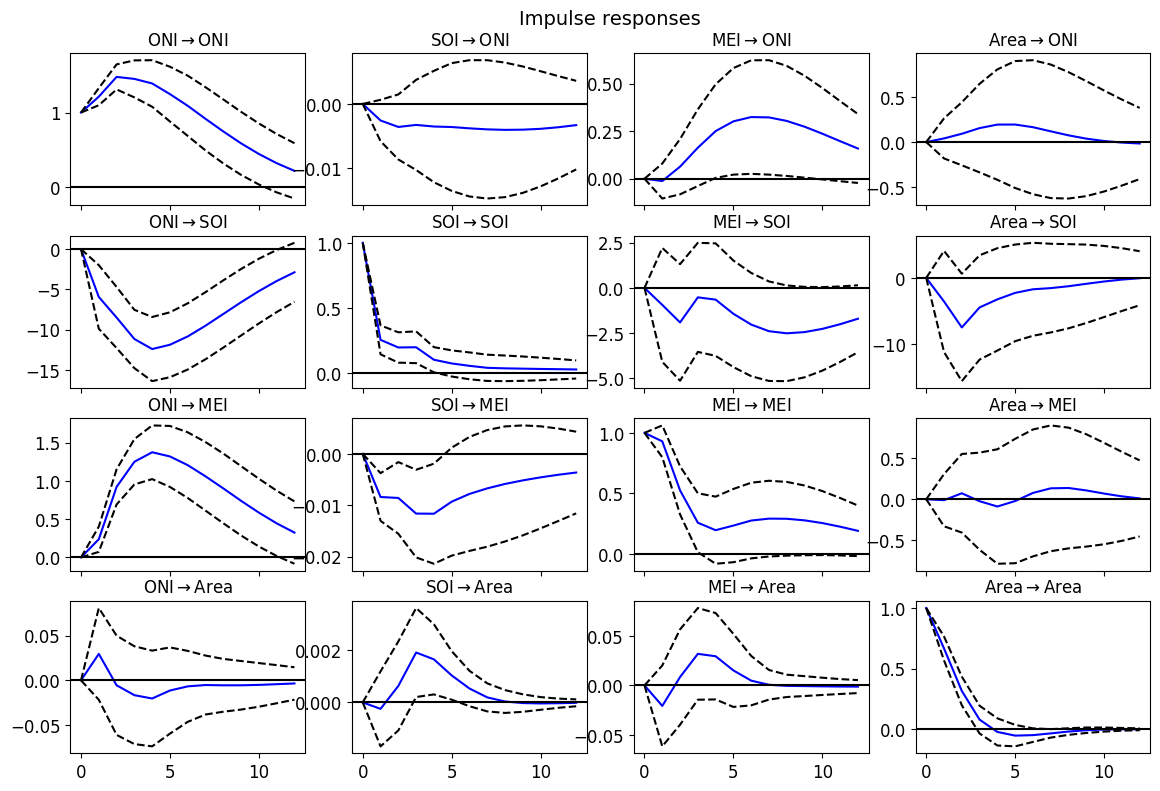
\includegraphics[scale=0.45]{Figures/var_ir.png}
    \caption{Funciones de respuesta al impulso (IRF) para el modelo VAR(3).}
    \label{fig:var_irf}
\end{figure}

\subsubsection{Conclusión parcial}
El modelo VAR(3) confirma la fuerte interrelación entre los índices ENSO (ONI, SOI, MEI) y muestra que la superficie de agua está particularmente influenciada por el SOI. Este resultado es consistente con la prueba de causalidad de Granger y con la lógica climática subyacente: la variabilidad atmosférica medida por el SOI tiene un efecto directo en la dinámica hidrológica del sistema estudiado. No obstante, la no normalidad de los residuos sugiere que futuros trabajos deberían considerar modelos más robustos (ej. VAR-GARCH o VAR con errores no gaussianos).


%----------------------------------------------------------------------------------------
%   SECTION 6: PRONÓSTICO ROLLING
%----------------------------------------------------------------------------------------

\section{Pronóstico rolling con SARIMA y VAR}

El pronóstico rolling permite evaluar la capacidad de los modelos para anticipar la evolución de las series en horizontes múltiples, actualizando el ajuste en cada paso con el valor observado. Este enfoque es más exigente que un pronóstico estático, ya que refleja el desempeño del modelo en un escenario de proyección operativa.

\subsection{Resultados con SARIMA}

La figura~\ref{fig:rolling_sarima} muestra el rolling forecast para la serie de \texttt{Área}. Se observa que el modelo sigue la dinámica general, aunque presenta limitaciones en la captura de picos abruptos. El modelo SARIMA fue evaluado usando las métricas:

\begin{itemize}
    \item MSE: 0,0133
    \item MAE: 0,0794
    \item RMSE: 0,1151
    \item MAPE: 43,07\%
\end{itemize}

Estos valores muestran un error moderado en términos absolutos (RMSE bajo), pero un MAPE elevado debido a la presencia de valores cercanos a cero, donde el porcentaje de error se amplifica.

\begin{figure}[H]
    \centering
    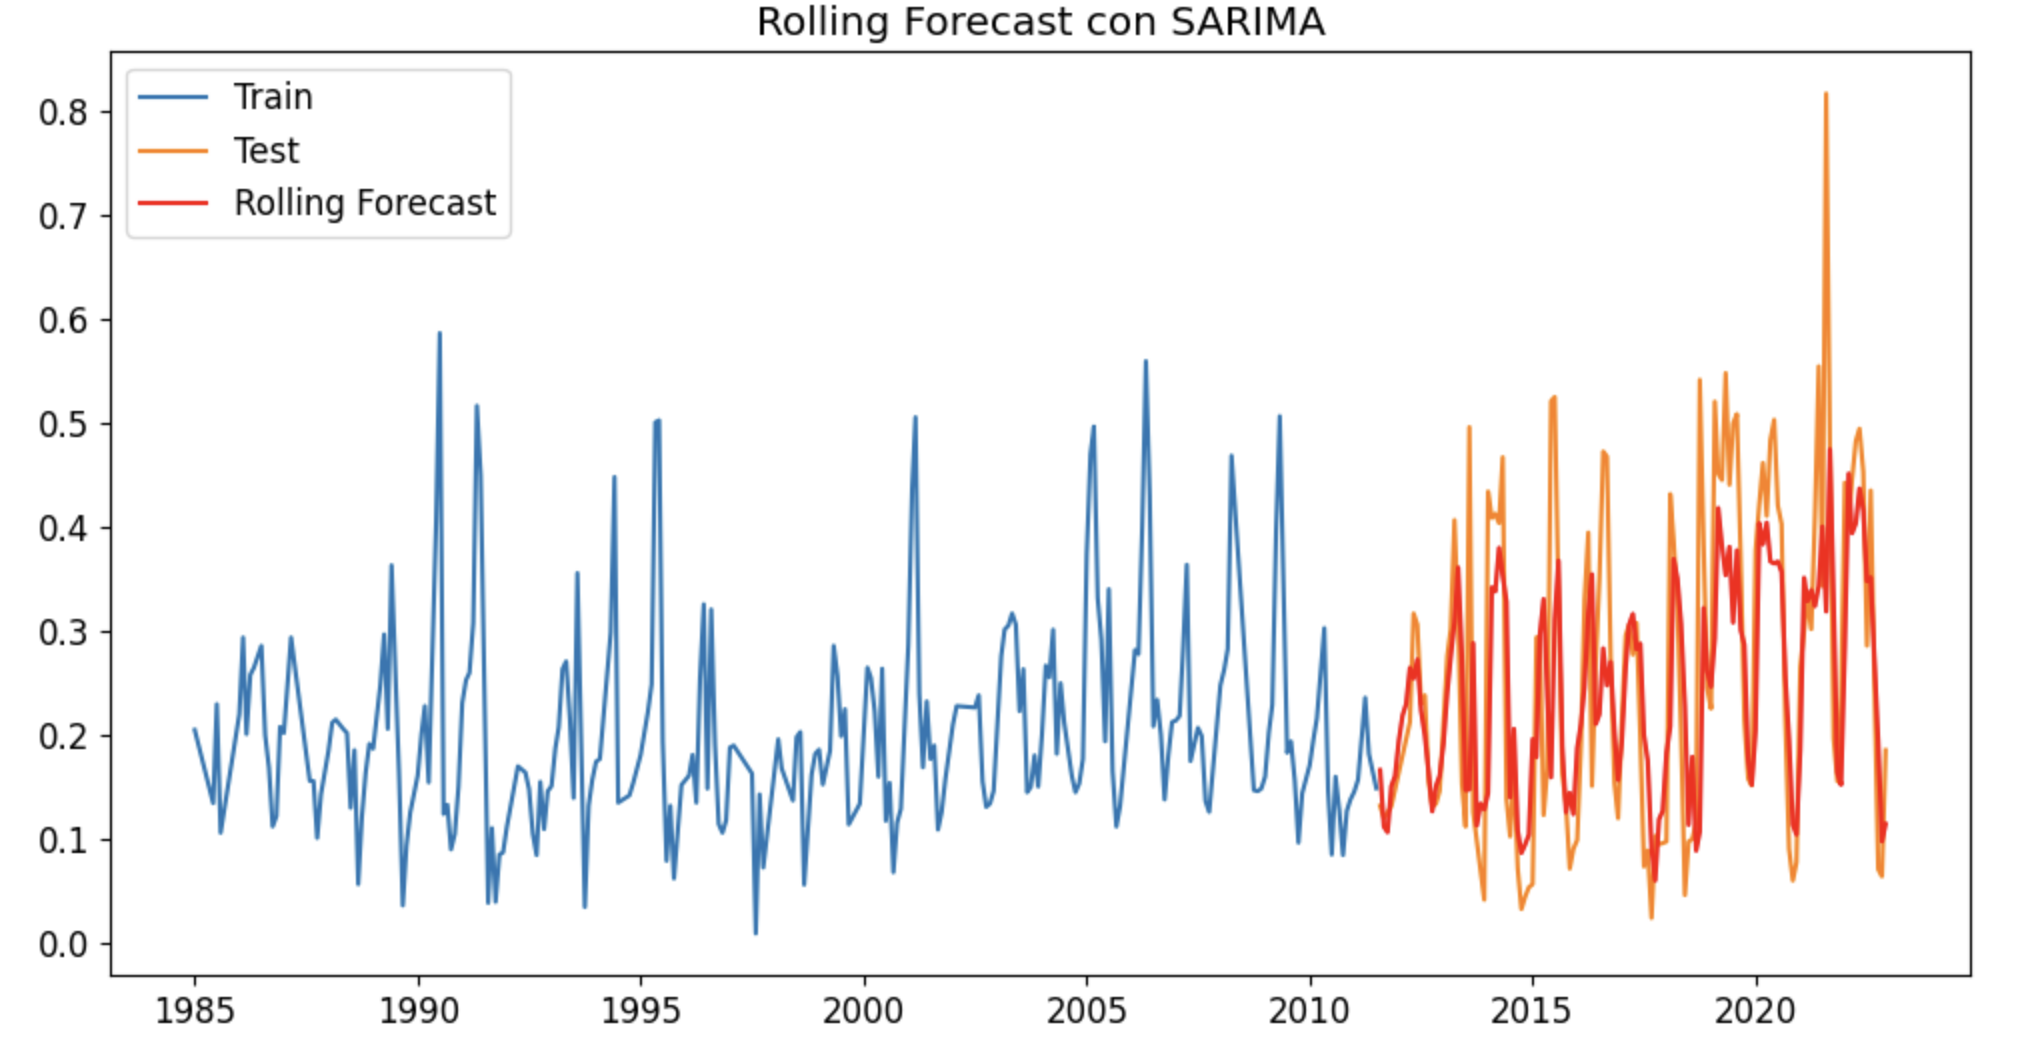
\includegraphics[scale=0.35]{Figures/rolling_sarima.png}
    \caption{Pronóstico rolling con SARIMA para la serie de Área.}
    \label{fig:rolling_sarima}
\end{figure}

\subsection{Resultados con VAR}

El modelo VAR fue evaluado para ONI, SOI, MEI y \texttt{Área}, con horizonte rolling de tres rezagos (figura~\ref{fig:rolling_var}).
La evaluación del modelo VAR dio los siguientes resultados:
\begin{itemize}
    \item MSE: 0,0176
    \item MAE: 0,0990
    \item RMSE: 0,1327
    \item MAPE: 45,58\%
\end{itemize}

\begin{figure}[H]
    \centering
    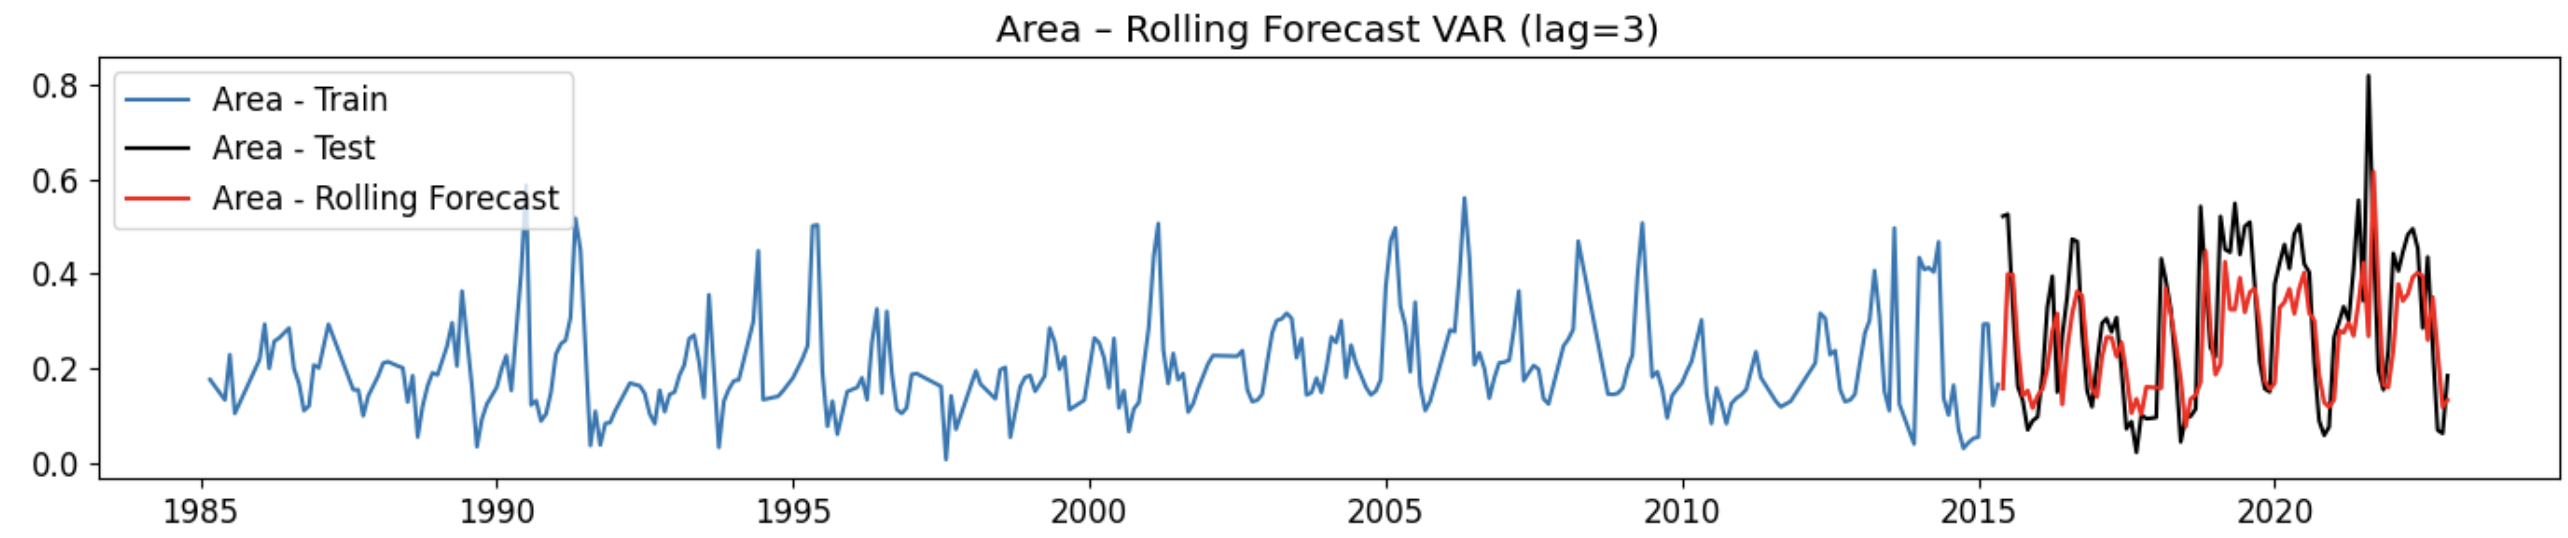
\includegraphics[scale=0.30]{Figures/rolling_var.png}
    \caption{Pronóstico rolling con SARIMA para la serie de Área..}
    \label{fig:rolling_var}
\end{figure}

\subsection{Comparación del desempeño en la serie Área}
La comparación de las métricas de la serie \texttt{Área} entre SARIMA y VAR muestra que ambos métodos alcanzan un desempeño satisfactorio, aunque con diferencias claras. El modelo SARIMA obtiene errores menores en todas las métricas (MSE = 0,0133; RMSE = 0,1151) frente al VAR (MSE = 0,0176; RMSE = 0,1327), lo que indica una mayor precisión en la predicción puntual, ver tabla \ref{tab:comp_area}. Asimismo, el MAE y el MAPE confirman la superioridad de SARIMA, reflejando que en promedio sus estimaciones se ajustan mejor a la magnitud real de la superficie de agua. No obstante, el VAR sigue mostrando un nivel de predicción aceptable, con la ventaja de modelar simultáneamente las interrelaciones con los índices ENSO, lo que lo convierte en una herramienta complementaria para analizar la dinámica conjunta del sistema climático-hidrológico.
\begin{table}[H]
    \centering
    \caption{Comparación de métricas para la serie Área entre SARIMA y VAR.}
    \label{tab:comp_area}
    \begin{tabular}{lcccc}
        \toprule
        Método & MSE & MAE & RMSE & MAPE \\
        \midrule
        SARIMA & 0,0133 & 0,0794 & 0,1151 & 43,07\% \\
        VAR    & 0,0176 & 0,0990 & 0,1327 & 45,58\% \\
        \bottomrule
    \end{tabular}
\end{table}


\subsection{Pronóstico espacio–temporal con CNN (U-Net temporal)}

Con el fin de extender el análisis hacia el futuro, se desarrolló un modelo de redes neuronales convolucionales capaz de predecir la presencia de agua en la laguna a partir de imágenes satelitales mensuales. Para ello se utilizó una variante de la arquitectura U-Net , adaptada para trabajar con secuencias de meses consecutivos en lugar de imágenes aisladas. De esta manera, el modelo aprovecha tanto la información espacial (formas y patrones dentro de cada imagen) como la temporal (cómo evoluciona el agua de un mes a otro).

El procedimiento consiste en entregarle al modelo un bloque de meses previos y pedirle que estime la máscara de agua del mes siguiente. Al repetir este proceso de manera encadenada (lo que se conoce como pronóstico autoregresivo), se obtiene una proyección de la dinámica de la laguna hacia adelante en el tiempo. Las salidas del modelo son tanto mapas de probabilidad de presencia de agua como máscaras binarias (agua/no agua) tras aplicar un umbral.

El entrenamiento se realizó con las series históricas de imágenes ya procesadas y normalizadas. Para evaluar su desempeño, se analizaron las curvas de pérdida en entrenamiento y validación, que mostraron una reducción estable a lo largo de las épocas. En los resultados cualitativos se observa que las predicciones del modelo reproducen coherentemente la forma y extensión de la laguna en distintos meses, mientras que la serie de área pronosticada mantiene la variabilidad temporal observada en los datos reales. En la figuras \ref{fig:forecast_cnn} y \ref{fig:forecast_cnn1} se pueden apreciar las predicciones con este método. 

Este enfoque basado en aprendizaje profundo permite no solo reconstruir el pasado de manera automática, sino también generar escenarios futuros de disponibilidad de agua en el salar, lo que constituye un aporte novedoso respecto a los métodos estadísticos utilizados en las secciones anteriores.

\begin{figure}[H]
    \centering
    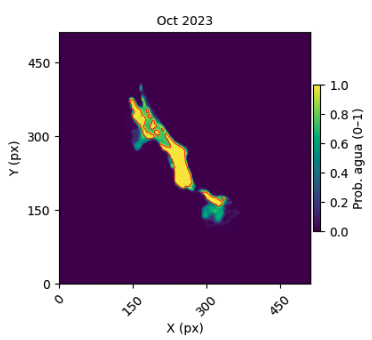
\includegraphics[scale=0.50]{Figures/forecast_cnn1.png}
    \caption{Pronóstico del área usando CNN (Octubre 2023).}
    \label{fig:forecast_cnn}
\end{figure}




\begin{figure}[H]
    \centering
    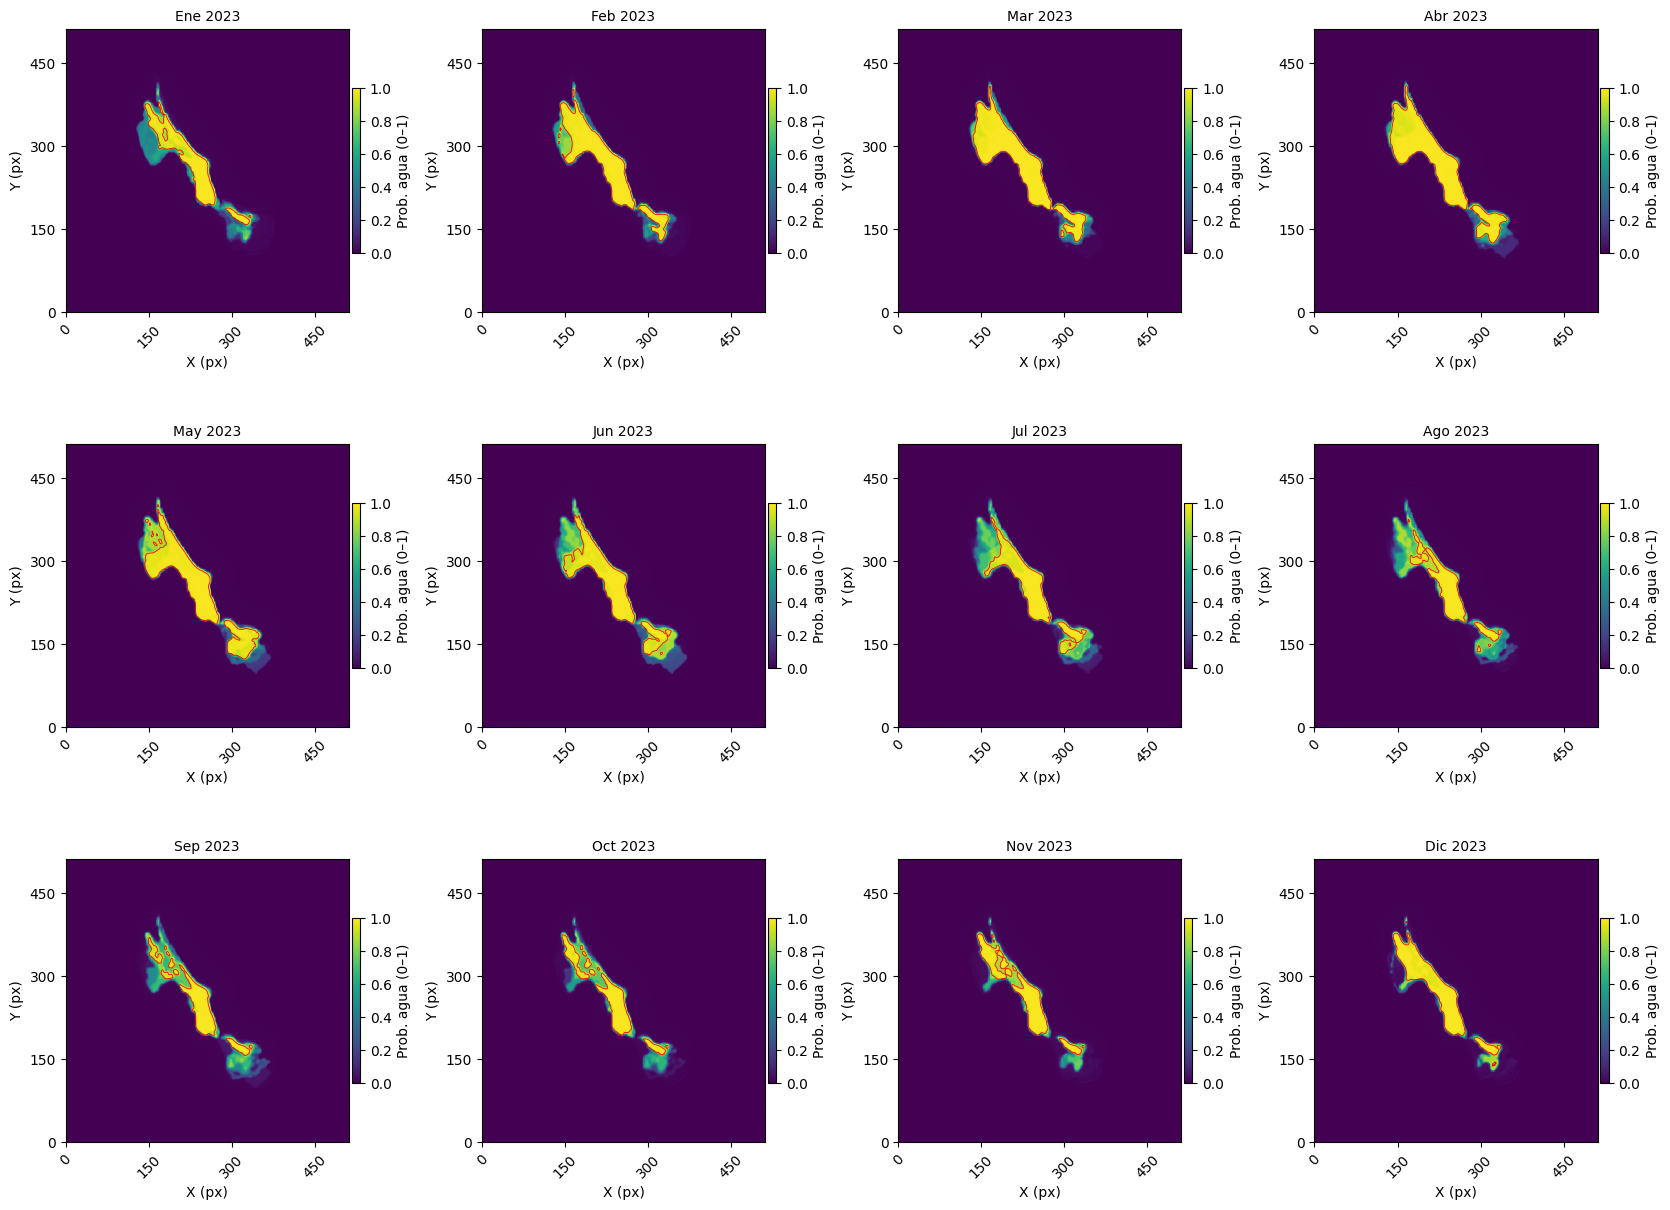
\includegraphics[scale=0.30]{Figures/forecast_cnn.png}
    \caption{Pronóstico del área usando CNN (12 meses).}
    \label{fig:forecast_cnn1}
\end{figure}

\subsection{Arquitectura de la U-Net temporal}

La arquitectura implementada corresponde a una variante de U-Net, adaptada para integrar secuencias mensuales de imágenes y generar predicciones espacio–temporales de la cobertura de agua. En este trabajo, la red se entrenó con ventanas de meses consecutivos y produjo como salida mapas de probabilidad de presencia de agua para el mes siguiente, que luego se umbralizaron para obtener máscaras binarias. El entrenamiento mostró curvas estables de pérdida, con valores finales bajos tanto en entrenamiento como en validación (figura~\ref{fig:curva_unet}), lo que evidencia una buena capacidad de generalización. En síntesis, la U-Net temporal permitió derivar series continuas de área de agua con coherencia espacio–tiempo, aportando una herramienta robusta para el pronóstico hidrológico del Salar de Llullaillaco.

\begin{figure}[H]
    \centering
    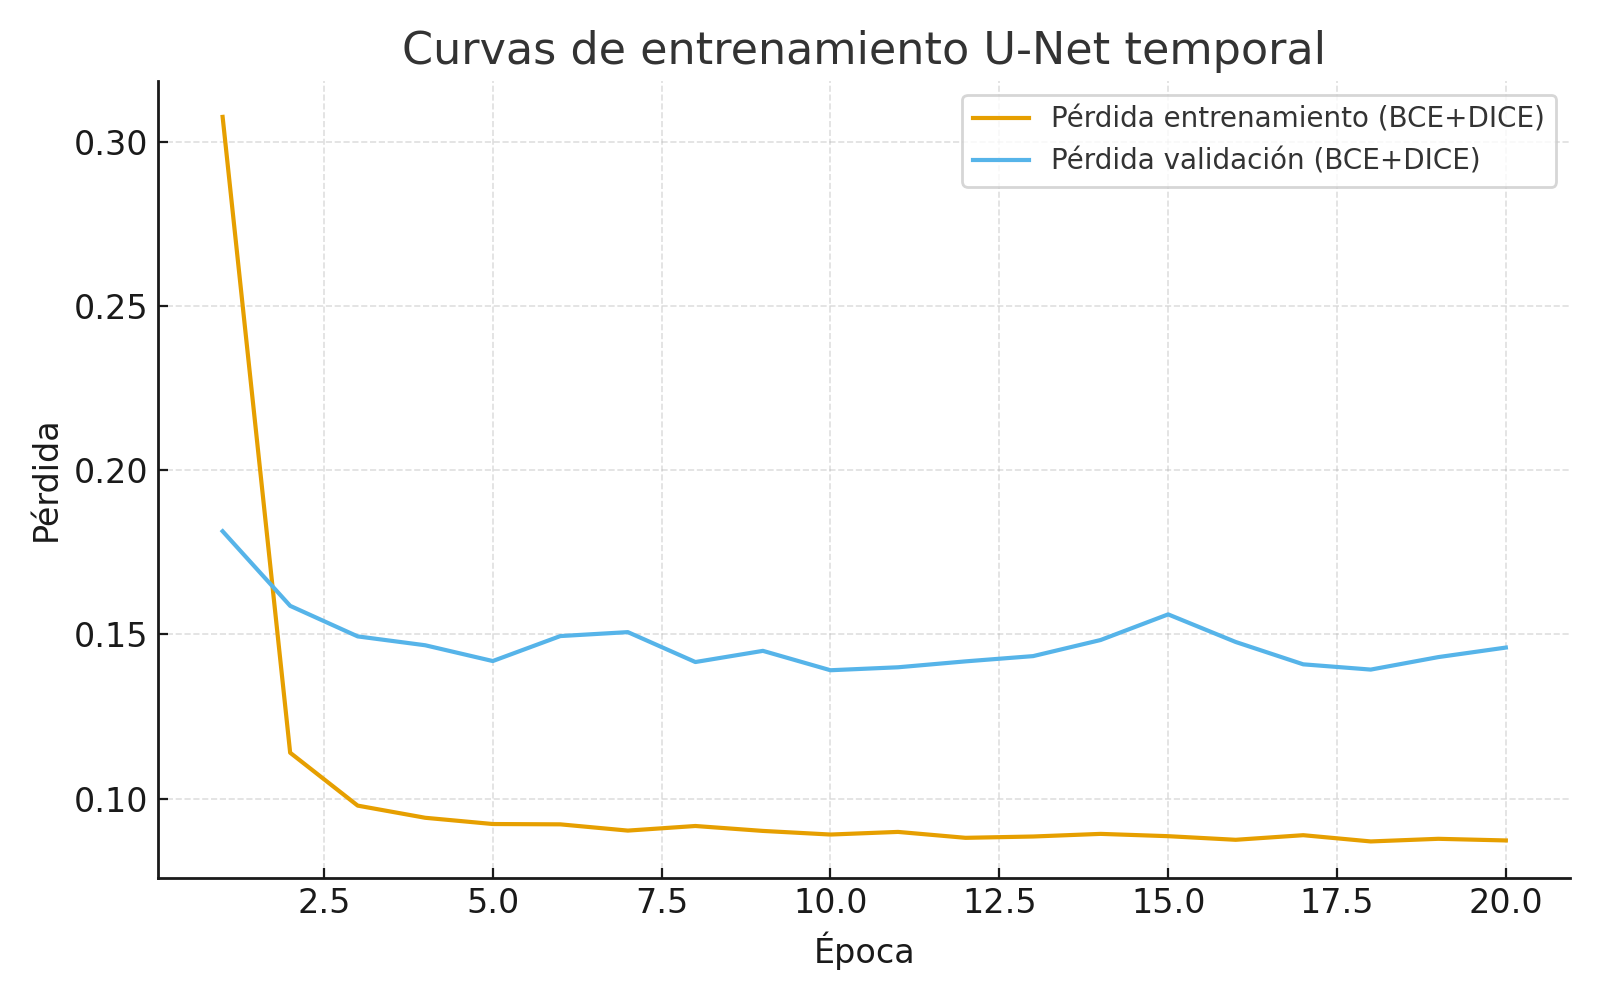
\includegraphics[scale=0.50]{Figures/curva_unet.png}
    \caption{Pronóstico usando CNN.}
    \label{fig:curva_unet}
\end{figure}




%----------------------------------------------------------------------------------------
% 4.4 LIMITACIONES Y OBSERVACIONES
%----------------------------------------------------------------------------------------
\section{Limitaciones y observaciones}
A continuación se detallan las principales limitaciones,  supuestos y riesgo del trabajo realizado.

\subsection{Cobertura y calidad de datos}
Respecto de la cobertura temporal, espacial y a la calidad de los datos, se pueden mencionar las siguientes limitaciones:
\begin{itemize}
    \item Brechas temporales y SLC-off: la falla del Scan Line Corrector (SLC) en Landsat 7 (post mayo 2003) y la transición 2012–2013 generaron huecos relevantes. Se mitigó con una estrategia híbrida (interpolación en brechas cortas y promedio estacional en brechas largas), pero persiste incertidumbre residual en esos intervalos.
    \item Máscaras y umbrales: la detección de agua depende del umbral NDWI ($>0.2$). Cambios razonables en el umbral o en el tratamiento de nubes/sombras pueden modificar el área estimada (sensibilidad a parámetros).
    \item Validación \textit{in situ}: no hubo verificación de campo, por lo que los umbrales y parámetros se justifican con literatura y coherencia interna; esto limita la cuantificación del sesgo absoluto.
\end{itemize}

\subsection{Supuestos estadísticos y diagnóstico de modelos}
Respecto de los modelos usados se mencionan las siguientes limitaciones asociadas a sus supuestos: 
\begin{itemize}
    \item Estacionariedad: ONI, SOI y MEI resultaron estacionarios por ADF, mientras que \texttt{Área} requirió diferenciación. El cumplimiento de estacionariedad es condición para SARIMA/VAR; desvíos locales pueden degradar el desempeño.
    \item Normalidad y heterocedasticidad de residuos: varios modelos (por ejemplo, ONI y MEI en SARIMA, y el VAR) muestran residuos no normales (colas pesadas) y, en casos, heterocedasticidad. Los intervalos de confianza deben interpretarse con cautela.
    \item Linealidad: Granger y VAR asumen relaciones lineales. Posibles no linealidades (o cambios de régimen) no modeladas pueden explicar parte del error, especialmente en picos del SOI.
    \item Métricas: el MAPE es poco informativo cuando hay valores cercanos a cero (índices ENSO). Se priorizaron RMSE/MAE y diagnóstico de residuos.
\end{itemize}

\subsection{Observaciones clave sobre resultados}
Como principales hallazgos en los resultados se mencionan:
\begin{itemize}
    \item Serie \texttt{Área}: la diferenciación mejoró la robustez y redujo el error validando el preprocesamiento.
    \item ENSO: fuerte interdependencia entre ONI, SOI y MEI (Granger), con un rol central del SOI sobre \texttt{Área}. El VAR confirmó persistencia propia de cada índice y efectos cruzados coherentes con la física climática.
    \item SOI: aunque los residuos no presentan autocorrelación relevante, las métricas de error del modelo SARIMA fueron altas respecto de su escala, sugiriendo simplificación y/o modelos alternativos (por ejemplo, con heterocedasticidad).
    \item Segmentación con U-Net: el etiquetado automático mediante la red permitió generar una serie temporal estable sin necesidad de anotación manual, aunque con limitaciones en la cuantificación de métricas exhaustivas de segmentación.
\end{itemize}


\subsection{Riesgos y mitigaciones}
Como principales riesgos y medidas de mitigación asociados a la modelación se detallan:
\begin{itemize}
    \item Dependencia de GEE y catálogos: fallos de disponibilidad pueden afectar la reproducibilidad. Mitigación: exportaciones imágenes.
    \item Sesgo por agregación espacial: el foco en la laguna central puede omitir dinámicas periféricas. Mitigación: probar la metodologia en otros sectores del salar.
     \item Complejidad computacional: el entrenamiento de modelos de segmentación y forecasting requiere recursos elevados. Mitigación: escalado progresivo, uso de subconjuntos y validación cruzada.
\end{itemize}



%----------------------------------------------------------------------------------------
% 4.5 CUMPLIMIENTO DE REQUERIMIENTOS
%----------------------------------------------------------------------------------------
\section{Cumplimiento de requerimientos}

El seguimiento de los requisitos definidos en la planificación muestra que se cumplieron satisfactoriamente en su mayoría. Entre ellos se incluyen: (i) descarga y procesamiento de datos satelitales desde GEE, (ii) modelado y predicción con SARIMA y VAR en tiempos operativos adecuados, (iii) visualización de mapas y series temporales, (iv) cálculo eficiente del NDWI, (v) métricas de precisión en la detección de agua, (vi) compatibilidad con formatos estándar (GeoTIFF y Shapefile), (vii) documentación técnica, y (viii) generación de reportes claros para usuarios. 

El único requisito pendiente corresponde a las pruebas con imágenes Sentinel-2, cuya validación cruzada se encuentra planificada pero aún no ejecutada. En síntesis, los requerimientos operativos de datos, modelado y visualización se encuentran cumplidos o muy avanzados, con un alto grado de replicabilidad.



